\documentclass{article}

\usepackage{fullpage,latexsym,picinpar,amsmath,amsfonts,graphicx, epstopdf } %}
%\epstopdfsetup{update}

\input{macros.tex}

\begin{document}
\centerline{REMOVED}
\centerline{REMOVED}
\centerline{\large \bf CS/MATH111 ASSIGNMENT 5}


\vskip 0.15in

%\noindent{\bf Individual assignment:} Problems 1, 2, and 3.
%\noindent{\bf Group assignment:} Problems 1, 2 and 3.

\vskip 0.15in


%%%%%%%%%%%%%%%%%%%%%%%%%%%%


\begin{problem}
An \emph{edge coloring} of a graph is an
assignment of colors to edges such that any two
edges that share an endpoint have different colors. (It can be proved that if the maximum vertex degree $D \ge 1$, then $G$ can be edge-colored with at most $2D - 1$ colors.)

Here is an example of an edge coloring of
a graph with $5$ colors (colors represented by numbers):

\begin{center}
\includegraphics[width=3.2in]{HW5_pics/graph_edge_color_hw5.pdf}
\end{center}

\noindent
For the graph above, find (show on the graph) an edge coloring with at most $4$ colors.



\end{problem}

%%%%%%%%%%%%%%%%%%%%%%%%%%%%
\begin{solution}

\begin{center}
\includegraphics[width=3.2in]{HW5_pics/problem1solution.pdf}
\end{center}

\end{solution}
%%%%%%%%%%%%%%%%%%%%%%%%%%%%

\begin{problem}
Let $G$ and $H$ be the graphs below. For each graph, determine
whether it is bipartite. 
If the graph is bipartite, determine whether it has a perfect matching.
Justify your answer.
%
\begin{center}
{\large Graph $G$:\ }
\begin{minipage}{2in}
        \includegraphics[width=2in]{HW5_pics/graph3_hw5.pdf}
\end{minipage}
\ \ \
{\large Graph $H$:\ }
\begin{minipage}{2.5in}
        \includegraphics[width=2.5in]{HW5_pics/graph4_hw5.pdf}
\end{minipage}
\hfill
\end{center}
\end{problem}


%%%%%%%%%%%%%%%%%%%%%%%%%%%%
\begin{solution}

G: The graph is not bipartite because the cycle g, f, e, i, d, g is of odd length.

H: The graph is bipartite with L = \{a,d,h,g,e\} and R = \{b,c,j,i,f\} and has perfect matching.

\begin{center}
\includegraphics[width=5.0in]{HW5_pics/HW5Solution2b.pdf}
\end{center}

\end{solution}
%%%%%%%%%%%%%%%%%%%%%%%%%%%%
\begin{problem}
Let G be the graph below. 
	\begin{center}
		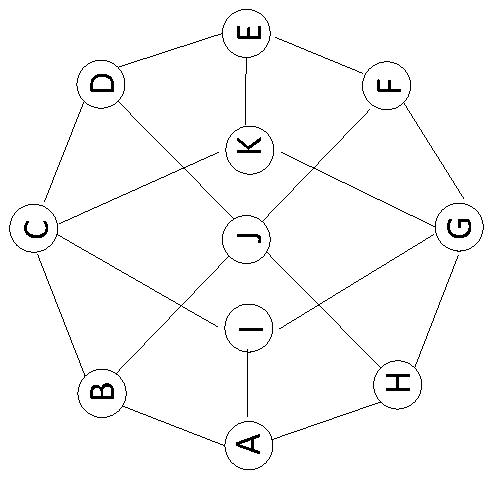
\includegraphics[angle = 270, width = 2in]{HW5_pics/Graph1HW5.eps}
		%\hfill
		%\includegraphics[width = 2.8in]{graphHa_hw5.pdf}
	\end{center}
	
\noindent (a) Determine whether it is bipartite. If the graph is bipartite, determine whether it has a perfect matching. Justify your answer.\\
(b) What is the chromatic number of G? Explain.\\
(c) Does G have a Hamiltonian Path? Justify.\\
(d) Is G a planar graph? (You need to either show a planar embedding or prove, that G is nonplanar.)
\end{problem}

%%%%%%%%%%%%%%%%%%%%%%%%%%%%
\begin{solution}

\noindent (a) The graph is bipartite with L = \{A,C,E,G,J\} and R = \{B,D,F,H,I,K\} however there is no perfect matching because 
there is an odd number of vertices so there is no set M of edges such that no two edges in M share an endpoint and every vertex has an edge that belong in M.

\begin{center}
\includegraphics[width=4.5in]{HW5_pics/HW5Solution3a.pdf}
\end{center}

\noindent (b) The chromatic number of G is 2 because this is the least number of colors needed so that no two adjacent vertices have the same color, as shown by the colored graph below.

\begin{center}
\includegraphics[width=4.5in]{HW5_pics/HW5Solution3b.pdf}
\end{center}

\noindent (c) There is a Hamiltonian Path: H,A,I,G,K,C,B,J,F,E,D

\begin{center}
\includegraphics[width=4.5in]{HW5_pics/HW5Solution3c.pdf}
\end{center}

\noindent (d) Yes, G can be redrawn as shown below:

\begin{center}
\includegraphics[width=4.5in]{HW5_pics/HW5Solution3d.pdf}
\end{center}

\end{solution}
%%%%%%%%%%%%%%%%%%%%%%%%%%%%


\begin{problem}
Determine which of the following two graphs is/are planar/nonplanar.
Justify your answer. (You need to either show a planar embedding or
use Kuratowski's theorem.)

	\begin{center}
		\includegraphics[width = 2.3in]{HW5_pics/graphGa_hw5.pdf}
		\hfill
		\includegraphics[width = 2.8in]{HW5_pics/graphHa_hw5.pdf}
	\end{center}

\end{problem}



%%%%%%%%%%%%%%%%%%%%%%%%%%%%
\begin{solution}
Graph G:
\begin{center}
\includegraphics[width=4.5in]{HW5_pics/HW5Solution4a.PNG}
\end{center}

When using Kuratowski's theorem and finding the subgraph, we end up with a subgraph that is homeomorphic to $k_5$ with vertices b, e, d, g, and a.
\newline

However, edges (e, d) and (b, g) intersect with each other, hence it is nonplanar.
\newline

Graph H: 
\begin{center}
\includegraphics[width=4.5in]{HW5_pics/HW5Solution4.pdf}
\end{center}

Graph H is planar as shown above.


\end{solution}
%%%%%%%%%%%%%%%%%%%%%%%%%%%%



\vskip 0.1in
\paragraph{Submission.}
To submit the homework, you need to upload the pdf file into ilearn and Gradescope.
Pictures should be imported into {\LaTeX} in pdf (see the source file to get an idea of how to do that). You can draw them in any drawing software and export in pdf, or draw by hand and scan.

\end{document}

